%
% File acl2015.tex
%
% Contact: car@ir.hit.edu.cn, gdzhou@suda.edu.cn
%%
%% Based on the style files for ACL-2014, which were, in turn,
%% Based on the style files for ACL-2013, which were, in turn,
%% Based on the style files for ACL-2012, which were, in turn,
%% based on the style files for ACL-2011, which were, in turn, 
%% based on the style files for ACL-2010, which were, in turn, 
%% based on the style files for ACL-IJCNLP-2009, which were, in turn,
%% based on the style files for EACL-2009 and IJCNLP-2008...

%% Based on the style files for EACL 2006 by 
%%e.agirre@ehu.es or Sergi.Balari@uab.es
%% and that of ACL 08 by Joakim Nivre and Noah Smith

\documentclass[11pt]{article}
\usepackage{acl2015}
\usepackage{times}
\usepackage{url}
\usepackage{latexsym}
\usepackage{amsmath}
\usepackage{bm}
\usepackage{graphicx}

\graphicspath{{figures/}}

%\setlength\titlebox{5cm}

% You can expand the titlebox if you need extra space
% to show all the authors. Please do not make the titlebox
% smaller than 5cm (the original size); we will check this
% in the camera-ready version and ask you to change it back.


\title{Predict of Helpfulness of Amazon Customer Review Using Deep Learning}

\author{Deliang Yang \\
  Electrical and Computer Engineering \\
  Michigan State University \\
  East Lansing, MI 48824 \\
  {\tt yangdeli@msu.edu} \\\And
  Nan Du \\
  Computer Science and Engineering \\
  Michigan State University \\
  East Lansing, MI 48824 \\
  {\tt dunan@msu.edu} \\}

\date{}

\begin{document}
\maketitle
\begin{abstract}
In this project, we are going to build a deep learning model to evaluate the helpfulness of Amazon customer product review. Gaining an incisive view on a product can always help customer make quicker and smarter purchase decisions. However, in reality, the number of products is tremendous, and the reviews vary a lot from one to another. This motivates us to build a model with state of the art deep learning techniques including LSTM and CNN to help customer to extract those really helpful product reviews. 
  
Extensive experiment are conducted in our evaluation, the results indicate the effectiveness of our proposed deep network model. We achieved 3\% higher than the previous work. We also explores how preprocessing and input data choice affect the test accuracy.
  
\end{abstract}

\section{Introduction}

Online Shopping is thriving and providing people convenient life and more product choices. Meanwhile, customer product views are abundant to help people purchase wiser and quicker. However, not all reviews contain useful and helpful information. Some reviews have more ``helpful" upvotes than the ``unhelpful" one but do not truly informative. What's more, personal, subjective, biased or emotional opinions and redundant information exist in many of the reviews we find below the product introduction, which wastes customers' time. As more and more powerful and interesting tools emerge in deep learning field, we would like to exploit some of the best that addressing natural language processing (NLP) to figure out what components would probably contribute to a high quality and useful product review. Such that we can identify them before a customer spending time reading it. 



We are going to employ both Long Short Term Memory (LSTM) RNN and Convolutional Neural Network (CNN) as our deep learning layout, applying to data collected on Amazon website to train our model, and the ground truth ``helpfulness'' will help us decide the helpfulness of a piece of review. 

The rest of the report is organized as follows. The related work will be addressed in Section 2. Technical approaches including deep network detail and preprocessing will be provided in Section 3. Data set information, evaluation results are shown in Section 4. Discussion on the results are in Section 5. Finally we conclude this paper. 

\section{Related Works}

The problem that why some review is helpful draws great attention for the researcher from business. Several projects were conducted to understand what are the main factors that determine the helpfulness of the customer review \cite{mudambi2010amazon,schindler2012peceivedhelpfulness}.

From the nature language processing perspective, people focus on how we can automatically to identify the helpful reviews. Different methods, including nonlinear regression \cite{liu2008nonlinear}, support vector machine \cite{kim2006svm}, and Random Forest method \cite{ghose2011randomforest} are applied to this problem. Recently, people start to adopt neural network model to analyze the problems. Multilayer perceptron neural network was successfully used to evaluate and predict the helpfulness of customer review on Amazon.com and Portuguese Steam Store \cite{mudambi2010amazon,barbosa2016steam}. The more complicated deep neural network model is also tested \cite{nguyevaluate2016lstm}. They achieve an accuracy of 65.0\% and an F1 score of 0.519.

\section{Technical Approach}

\subsection{Preprocessing}

\subsubsection{Tokenization}\label{tech_token}

Since computer can only handle with numbers instead of texts, we need to tokenize the words in sequence before feeding it to the deep network model. First, we add each unseen word to a dictionary. For those words already in the dictionary, the corresponding value will increment 1. Second, after the whole dataset is traversed, the dictionary is sorted based on the word count. Most frequent words will has a small token number, starting from 1, like ``the'', ``a'', etc. The number 0 is reserved for those unseen or infrequent words, which means ``unknown''. Finally, another dictionary that stores the token of each word for reference is built.

\subsubsection{Word Embedding}

Word embedding is a common approach to assign meaningful values to the word tokens. For traditional nature language processing task, the systems traditionally treat words as discrete atomic symbols. The learning model only have little knowledge about the words use such arbitrary encoding without discover the relationship exist between the individual symbols. Representing words as unique, discrete ids furthermore leads to data sparsity. Usually such case means that we may need more data in order to successfully train statistical models. To overcome these obstacles, using vector representations is necessary. Also, the dimension of embedding is scalable, we can choose the appropriate dimensions according to the size of token of the application. Next, vectors can be compared via different approaches. For example, cosine proximity can capture the similarity between two vectors, ``coconut'' and ``tripod'' should have low similarity, but ``dinner'' and ``kitchen'' shall be close.\\

\paragraph{Word2vec} \cite{mikolov2013word2vec} is a particularly computationally-efficient word embeddings model for learning from raw text. There are two major underlying approaches, the Continuous Bag-of-Words model (CBOW) and the Skip-Gram model. CBOW predicts target words from source context words, while the skip-gram predicts source context-words from the target words. When we have larger dataset, the skip-gram schemes tends to generate better result, as it treats each context-target pair as a new observation. We follow the tutorial from Google TensorFlow and focus on train a model based mainly on skip-gram \cite{word2vectutorial}.

In skip-gram model, current word is treated as an input to a log-linear classifier with continuous projection layer, and generate prediction on words within a certain range before and after the current word. The model give distant word less weighting by sampling less as usually such words not strong related to the current word.

Loss function of our training is calculated by compare the observed examples and noisy examples. The embeddings is updated by taking a small step in the direction of the gradient. When this process is repeated over the entire training set, the embedding vectors will move around for each word until the model is successful at discriminating real words from noise words.\\

\paragraph{GloVe} For our neural networks, we use pre-trained GloVe embedding model \cite{pennington2014glove} to generate embedding of our input. GloVe is a global log-bilinear regression model trained on non-zero entries of a global word-word co-occurrence matrix, which stores the information of how frequently words co-occur with one another in a given dataset. The pre-trained model is trained by Wikipedia 2014 and Gigaword 5 as corpus. The corpora have 6,000,000,000 tokens with 400,000 words. The pre-trained model has 100-dimensional embeddings.

\subsection{Recurrent Neural Networks}

The major method we are using is deep learning. \textbf{Recurrent Neural Networks}, or RNNs \cite{rumelhart1986} are the family of the deep learning structures to process sequential data. Parameter sharing across the different parts of the model is the key idea that makes RNNs to be able to deal with the sequential data. Specifically, the RNNs we talked about is operating on a sequence that contains vectors \(\bm{x}^{(t)}\) with the time step index t ranging from 1 to \(\tau\).

A simple recurrent neural network will just process the information from the input \(\bm{x}\) and incorporate it into the state \(\bm{h}\) of hidden unit and  passed to the next unit. The hidden unit state \(\bm{h}\) at time step t, \(\bm{h}^{(t)}\),
\[\bm{h}^{(t)} = f(\bm{h}^{(t-1)},\bm{x}^{(t)}; \bm{\theta} )\]
RNN also usually have extra architectures like output layers that output the result of \(\bm{h}\) for further processing or predictions.

\begin{figure}[htbp]
	\centering
	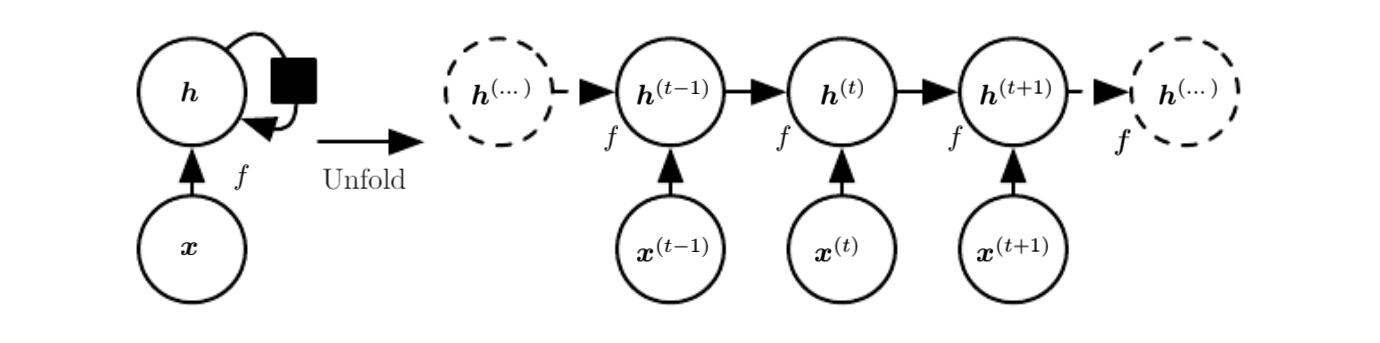
\includegraphics[width=0.9\linewidth]{SimpleRNN.jpg}
	\caption{A simple recurrent neural network structure without output.}
	\label{fig:rnn}
\end{figure}

We can use a function \(g^{(t)}\) to represent the unfolded recurrence after t steps, given us another representation of \(\bm{h}^{(t)}\),
\[\bm{h}^{(t)} = g^{(t)}(\bm{x}^{(t)}, \bm{x}^{(t-1)}, ...\bm{x}^{(2)}, \bm{x}^{(1)})\]

In this form, \(g^(t)\) takes the input of whole past sequences \((\bm{x}^{(t)}, \bm{x}^{(t-1)}, ...\bm{x}^{(2)}, \bm{x}^{(1)}))\) as input and output the current state. However, we can unfolding the structure and repeated apply function \(f\) to achieve same output. By doing this we can use the same transition function \(f\) with the same parameters at every step.

However, a simple RNNs cannot learn long time dependency as in the optimization. As we described above, at each time step we repeatedly apply the same operation \(f\). We can use a multiplication on matrix \(\mathbf{W}\) to represent such operation. Suppose that matrix \(\mathbf{W}\) has an eigendecomposition \(\mathbf{W} = \mathbf{V}\textnormal{diag}(\bm{\lambda})\mathbf{V}^{-1}\). After $t$ steps, the input already multiply \(\mathbf{W}^{t}\), so:
\[\mathbf{W}^{t} = \mathbf{V}\textnormal{diag}(\bm{\lambda})^{t}\mathbf{V}^{-1}\]
Means that given enough large steps t, any eigenvalue\( \lambda\) that not close to 1 will either vanish (less than 1) or explode (larger than 1). The gradient in such graph also scaled according to \(\textnormal{diag}(\bm{\lambda})^{t}\) \cite{goodfellow2016deeplearning}. In this case, it difficult to optimize such gradient as it hard to know the direction at near 0 gradient and learning with explode gradient is unstable. To solve this challenge, gated RNNs is proposed and becomes one of the most effective practical models that used for sequential data.\\

\subsubsection{Introduction to LSTM Unit} \cite{hochreiter1997lstm} is one branch of such gated RNNs that is extremely successful in the application like speech recognition, machine translation, and handwriting generation. The key idea of LSTM is to introduce a self loop so that gradient can flow for long duration. 

The self loop (internal recurrence) is located in ``LSTM cells'' with outer recurrence like ordinary recurrent network. The cell is controlled by a combination of input gate and memory control gates, formulated by equations below.

\begin{align*}
	&i_t = \sigma(U_ih_{t-1}+W_ix_t + b_i)\\
    &f_t = \sigma(U_fh_{t-1}+W_fx_t + b_f) \\
    &o_t = \sigma(U_oh_{t-1}W_ox_t + b_o) \\
	&\tilde{c} = \sigma(W_cx_t + U_ch_{t-1}+b_c)\\
	&c_t = f_t\odot c_{t-1} + i_t \odot \tilde{c}_t \\
	&h_t = o_t\odot \sigma(c_t)
\end{align*}

where $i_t$, $f_t$ and $o_t$ are three gates that control input, forget and output respectively. Each of the gate output signal depends on its state transition matrix $U$, input weighting matrix $W$ and bias $b$. The final cell state $c$ is updated by element-wise multiplication, denoted by operator ``$\odot$''. $\sigma$ is the activation function, which can be chosen from sigmoid, ReLU, tanh and so on. 

As we can see, LSTM adds two more gates to control the output and previous inputs, thus has the ability to capture the long term dependencies in the sequence. 


% The self loop (internal recurrence) is located in ``LSTM cells'' with outer recurrence like ordinary recurrent network. The weight of self-loop is controlled by a forget gate $f_i^{(t)}$:

% \[f_i^{(t)} = \sigma (b_i^f + \sum_{j}U_{i,j}^f x_j^{(t)} +\sum_{j}W_{i,j}^f h_j^{(t-1)} ) \]

% where $\boldsymbol{x}^{(t)}$ is the current input vector and $\boldsymbol{h}^{(t)}$ is the current hidden layer vector, containing the outputs of all the LSTM cells. $\boldsymbol{b}^f$, $\boldsymbol{U}^f$, and $\boldsymbol{W}^f$ are biases, input weights, and recurrent weights of the forget gate, respectively. The internal state of LSTM cell is updated with the following equation:

% \begin{small}
% \[s_i^{(t)} = f_i^{(t)}s_i^{(t-1)}+g_i^{(t)}\sigma(b_i + \sum_{j}U_{i,j}^f x_j^{(t)} +\sum_{j}W_{i,j}^f h_j^{(t-1)} )\]
% \end{small}

% And the external input gate unit 
% \(g_i^{(t)} \)
% is computed with the following equation:
% \[g_i^{(t)} = \sigma (b_i^g + \sum_{j}U_{i,j}^g x_j^{(t)} +\sum_{j}W_{i,j}^g h_j^{(t-1)} ) \]
% The output 
% \(h^{(t)}\)
% and the output gate 
% \(q_i^{(t)}\)
% , are updated using sigmoid function also:
% \begin{eqnarray*}
% h_i^{(t)} &=& \tanh (s_i^{(t)})q_i^{(t)}\\
% q_i^{(t)} &=& \sigma (b_i^o + \sum_{j}U_{i,j}^o x_j^{(t)} +\sum_{j}W_{i,j}^o h_j^{(t-1)} )
% \end{eqnarray*}

LSTM is proven to be able to learn long-term dependencies more effectively than normal RNNs. In our project, we will use LSTM as our main method. We also plan to compare LSTM performance with other network structures.

\subsubsection{LSTM Network Model}

In our design, the core part is the LSTM layer. LSTM with 256 units is the feature extractor that processes the sequence. The recurrent activation function is \texttt{tanh}.  Besides LSTM network, we add two important layers in the network. Before LSTM layer we employ the \texttt{Embedding} layer, which embeds the token with the corresponding vectors. After the LSTM layer, a dense (fully connected) layer with 50 units is added. Finally, a 3-unit dense layer with \texttt{softmax} activation is used to extract the label of the sequence.

\subsubsection{LSTM in Regression}

In regression part, we try to predict the helpfulness score from the given sequence. Intuitively, using merely two or three classes to separate the data will definitely result in coarse granularity. However in regression, the output will be a continuous number, which yields fine granularity.  Actually if we calculate the helpfulness score by helpful upvotes over the total votes, we get different number ranging from 0 to 1. 

In regression part, the final dense layer will only have one unit, with linear activation. The loss function are changed to cosine proximity correspondingly to compare the correlation coefficient of the predicted score vector and the true vector.

\subsection{Convolutional Neural Networks}
One of the most successful model in recent years is Convolutional Neural Networks (CNNs). The major difference between CNNs and traditional neural networks is to replace the general matrix operation in the tradition layer with the mathematical operation called convolution, shown in the following equation:
% \paragraph{Convolution operation}
% In mathematics, the convolution of function \(x\) and \(w\), \(s(t)\), is defined as following equation:
\[s(t)=\int x(a)w(t-a)dt = (x * w)(t)\]

% In convolutional network terminology, the first argument (in this example, the function x) to the convolution is often referred to as the input and the second argument (in this example, the function w) as the kernel. The output is sometimes referred to as the \textit{feature map}.

% The convolution operation in the matrix can treat as a kind of matrix multiplication. As the Figure 1 shower, the kernel convolution take source pixel from input matrix and simply multiplied the kernel matrix to generate the element for the convolutional layer output.\\

% \paragraph{Major feature of CNNs} 
There three major features that make CNNs so successful: sparse interactions, parameter sharing, and equivariant representations.

Sparse interactions mean that the neuron in the convolutional layers only needs to interact with several neurons in the input and output layers. In the contrast, a neuron in the traditional neural network needs to interact every neuron in the input and output layers. In this way, the CNNs can easily learn some small and meaningful features which are only from tiny part of the input matrix. Also, it can save a lot of computation time.

Parameter sharing refers to using the same parameter for more than one function in a neural network. At every position of the input in CNNs, it will use the each element of the kernel matrix. By doing this, the layer can learn something with a whole picture.

Equivariant representations describe the phenomenon that if the output will change corresponding to the change of input. \\

% \paragraph{Add pooling layer} When we obtained the output from convolutional layers, sometimes we will apply another layer model called pooling layer to modify the output further.

% One of the popular pooling operation is called max pooling and Figure 2 shows an example of how the operation will work on the matrix.

% The pooling operation will help CNNs be more robust to the tiny translation from the input, which we called invariance to local translation. This can be a useful property if we care more about whether some feature is present rather than its exactly location. \\

\subsection{CNN for text classification}
For a word, we can use a k-dimension vector \(\bm{x}\) to represent it. So a sentence of length n is represented as:
\[\mathbf{x}_{1:n} = \bm{x}_1 \oplus \bm{x}_2 \oplus ... \oplus \bm{x}_n\]
Here operator \(\oplus\) is the concatenation operator. We applied convolution filter \(w\) on a window of size h, to transform the input \(\mathbf{x}_{1:n}\) to a new feature \(c_i\):

\[c_i = f(\mathbf{w}\cdot\mathbf{x}_{i:i+h} + b ) \]
 Here b is the bias term and f is the activation function usually using non-linear function like sigmoid or hyperbolic tangent. By repeated apply the operation, we can finally generate feature map. Then the max-over-time pooling was applied to keep the most important features.
 
In the model, we apply multiple filters with varying window size, to extract multiple features\cite{kim2014cnntext}. These features then used as input for a fully-connected layer and then convert to the probability of labels.\\

\paragraph{Highway structure} We also add a highway structure \cite{srivastava2015highway} in our model. The highway structure allows unimpeded information flow across several layers. It uses gating units to learn to regulate the flow of information through the network. In our model, the highway structure is used to connect different CNNs with the different filters.

\section{Evaluation}

\subsection{Data Set}

The data set we use is available on \url{http://jmcauley.ucsd.edu/data/amazon/} website. There are reviews from many categories, such as books, electronics, sports, toys and so on. As we know, review towards product from different categories will show different patterns. So, in this project we may probably focus on only one category, which is electronics product reviews. If the result is remarkable, we can apply a similar model to other sets. 

The electronics review database has more than 1.68 million reviews. Each piece of review is in \texttt{.json} format, consisting of fields like \texttt{reviewerID}, \texttt{productID}, \texttt{helpful}, \texttt{reviewText}, \texttt{overall rating}, \texttt{summary}, \texttt{reviewTime} and so on. One can check the website for more information. 

In evaluation, we manually categorize the review into 3 different classes, which are Neutral, Helpful and Unhelpful. If a review has no votes or the number of helpful votes is equal to unhelpful votes, then the review is Neutral. Else if the helpful votes outnumbers the unhelpful ones, then it is helpful, otherwise it's unhelpful. Statistical results show that more than half of the reviews have no votes. The proportions of each category are 60\%, 32\% and 8\% for Neutral, Helpful and Unhelpful respectively. 

\begin{figure}[tbp]
    \centering
    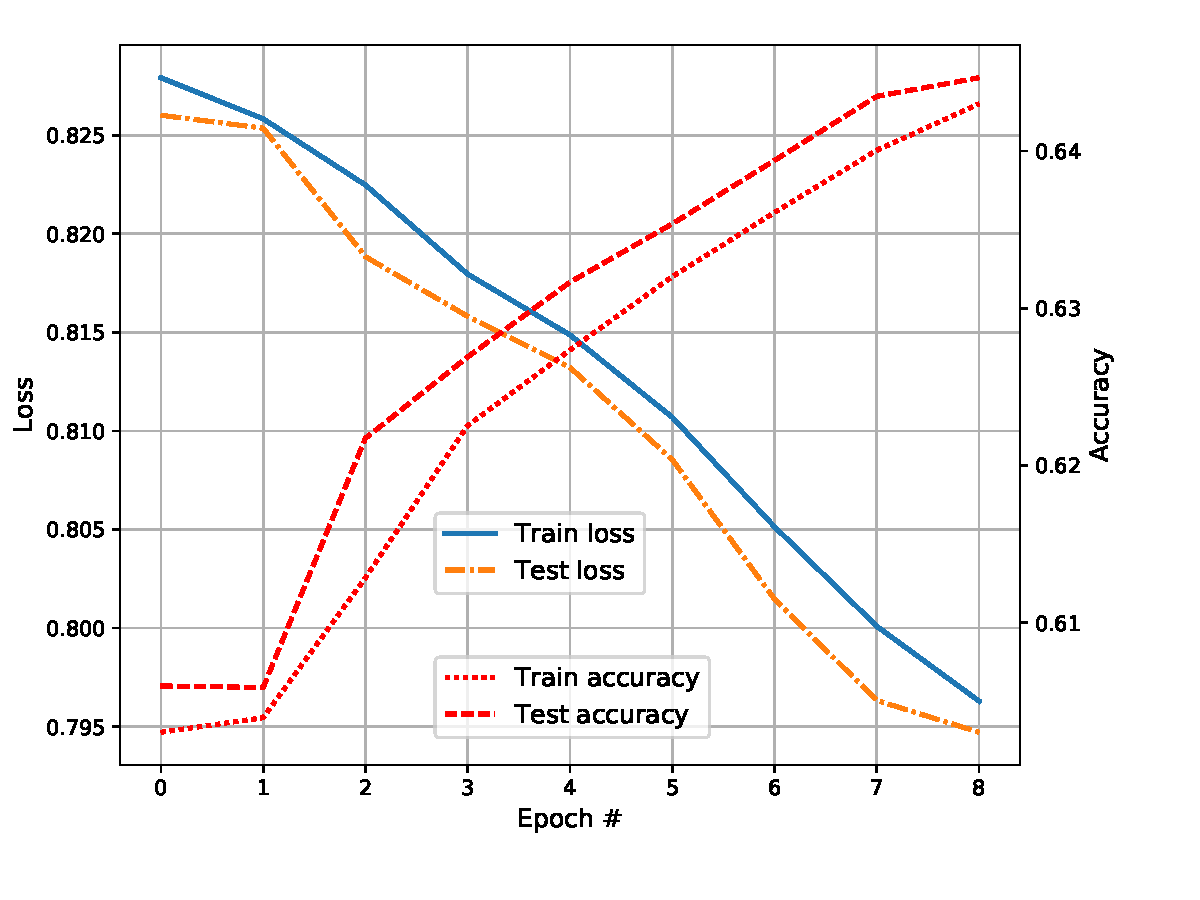
\includegraphics[width=\linewidth]{./figures/hpcc_train_loss_acc.pdf}
    \caption{Training and testing accuracy and loss of the baseline.}
    \label{result_loss_acc}
\end{figure}

\subsubsection{Tokenization}

With the tokenization method mentioned in Section \ref{tech_token}, 551,152 unique tokens have been recorded out of the total 196 million tokens. However over 85\% percent of the tokens are typos, model names or number sequence, which introduces noise to the data set. We can do stop word removing and stemming, but it is left for future work. 

\subsubsection{Vectorization}

In vectorization process, the embedding matrix manages to identify 88,327 tokens out of the 551k unique tokens, which means the majority of the tokens are not addressed. In that case, the tokens are embedded by a 100-dimensional vector.

\subsection{LSTM Classification Results}

We implement the proposed network layer via \texttt{Keras}, using \texttt{Tensorflow} as backend. The benchmark is conducted by feeding all the samples in the corpus on High Performance Computing Center (HPCC) platform in Michigan State University. Since it takes all samples into account, it is expected to higher accuracy than small sample sizes. After 8 epochs, the test accuracy reaches 64.0\%. The training and testing results can be seen in Fig. \ref{result_loss_acc}. In Fig. \ref{result_acc_comp}, we compare our result with other work. Previous work with 2 layers LSTM achieves the best test accuracy at 65\%, which is slightly higher than our baseline. We use another two traditional approaches as comparison, k-Nearest Neighbor (kNN) and simple RNN. As we can see, the kNN method can not achieve high accuracy, indicating that distance based classifier has trouble in handling sequence data. For simple RNN, since it don't have long term memory, the test accuracy is lower than the LSTM models. 

\begin{figure}[tbp]
    \centering
    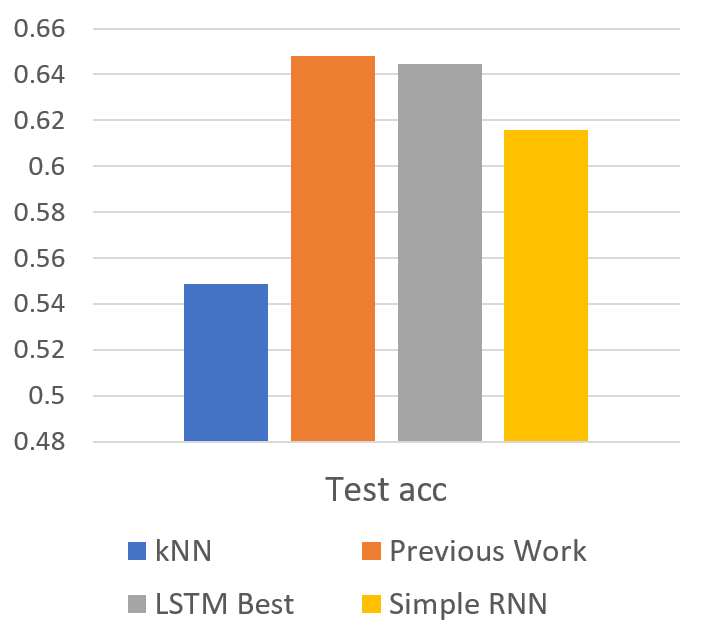
\includegraphics[width=0.9\linewidth]{./figures/acc_comp.png}
    \caption{Accuracy comparison between the LSTM model and previous work.}
    \label{result_acc_comp}
\end{figure}

Unfortunately, in our experiment, we notice that the model needs too much time to train a epoch. So we use small dataset, which contains 65,535 samples, as our small size evaluation, which is easier to compare the results from different configurations. The baseline for the smaller dataset is lower than the whole one, around 61.5\%. 

In the first setup, we explore how preprocessing affects the final performance. Hence two different experiments are conducted. The first one is pre-padding, which appends 0 vectors as prefix of the sentence with sequence length less than 256 (we use post-padding by default). The second one removes the word vector embedding, using only the tokenized sample as input. The corresponding results is in Fig. \ref{result_acc_f1_comp_pp}. As one can notice, changing the padding of the sequence has large influence on the performance,  leading to a 4\% drop in the accuracy. However, the effect of vector embedding is not as good as our expectation. Without vectorization, the accuracy deceases only by 1.5\%. 

\begin{figure}[tbp]
    \centering
    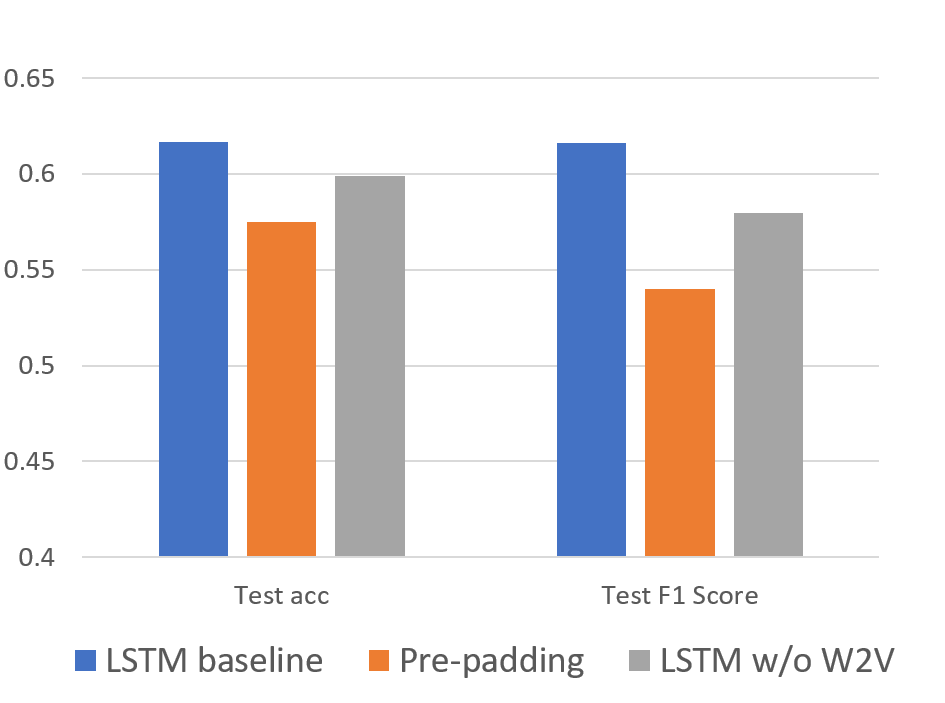
\includegraphics[width=0.9\linewidth]{./figures/acc_f1_comp_pp.png}
    \caption{Comparison of accuracy and F1 score by changing preprocessing.}
    \label{result_acc_f1_comp_pp}
\end{figure}

In the second setup, we alter the input data. There are 4 experiments conducted, as listed below:

\textbf{Remove the review with 0 votes}. The review with 0 votes consist of half of the total samples. The removal of them can balance the data, however, helpful reviews also outnumber the other two categories in the remaining samples. So the dataset is still biased.

\textbf{Binary classification with biased data}. In this case, we merge the Neutral data to the unhelpful ones, such that there are only two categories. The network structure is also altered to accommodate this. The 3-unit dense layer is replaced by a one-unit dense layer with sigmoid function. 

\textbf{Binary classification with balanced data}. Now we have a dataset with equal number of helpful and unhelpful review by shrinking the size of helpful review.

\textbf{Binary classification with balanced data achieved by changing threshold}. Here we change the decision boundary manually to achieve equal sample size. 

The results for the above 4 cases are plotted in Fig. \ref{result_f1_comp_ip}. After the removal of the 0-vote reviews, there is a 20\% boost from the baseline cases. We suppose that those 0-vote reviews may potentially be helpful (or unhelpful). They are just not seen by many customers. After all, not every customer would upvotes a review. Thus we can not obtain accurate ground truth. That's one possible reason for the boost in accuracy after the removal. In the next case, when the neutral review are merged into the unhelpful one, the accuracy remains almost the same. However, the F1 score increases by 10\%. Because in this case we have higher recall, but the precision decreases. In case 3 where we balance the number of two categories, the test accuracy and F1 score, surprisingly, is lower than the baseline. Yet we don not have a clue about the reason. Finally, the result from data set achieved by changing the threshold indicates that the test accuracy remains the same as the baseline case, but the F1 score increase by about 9\%. 

The results above illustrate that precise ground truth plays an important role in our evaluation and is more important than a balanced dataset. 

\begin{figure}[tbp]
    \centering
    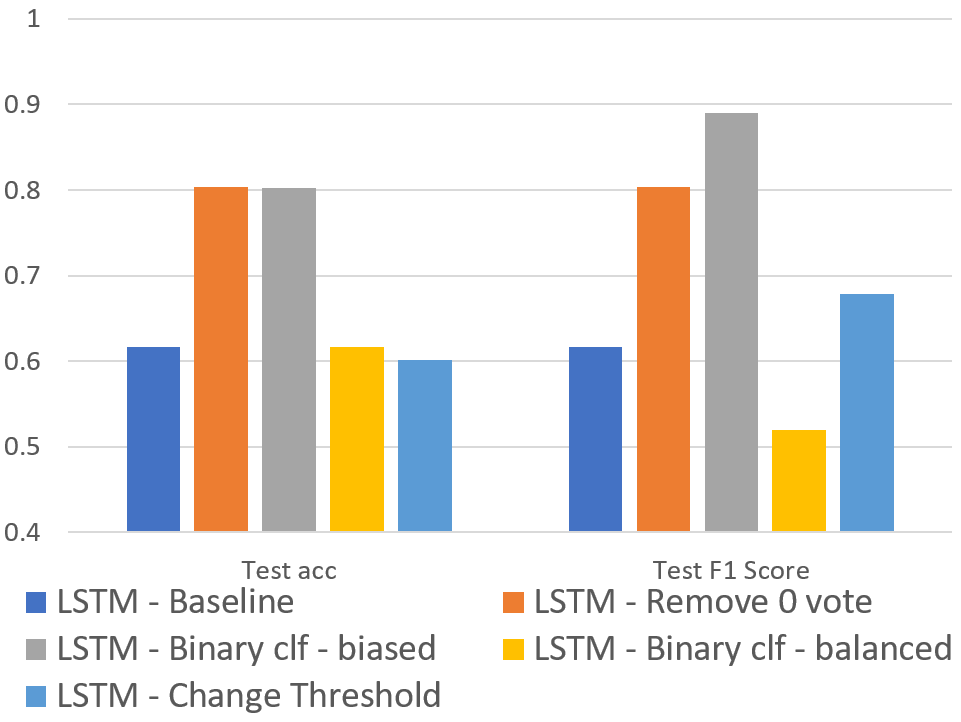
\includegraphics[width=0.9\linewidth]{figures/acc_f1_comp_ip.png}
    \caption{Comparison of accuracy and F1 score by changing input.}
    \label{result_f1_comp_ip}
\end{figure}

\subsection{LSTM Regression Results}

For the regression part, after using the original dataset as benchmark, we would carry out two experiments regarding the input. The first case is the same as one in the classification section, which is remove the 0-vote reviews. The other one is actually based on the data after the removal, adding a penalty at the helpfulness score. The penalty is define as 

\begin{figure}[tbp]
    \centering
    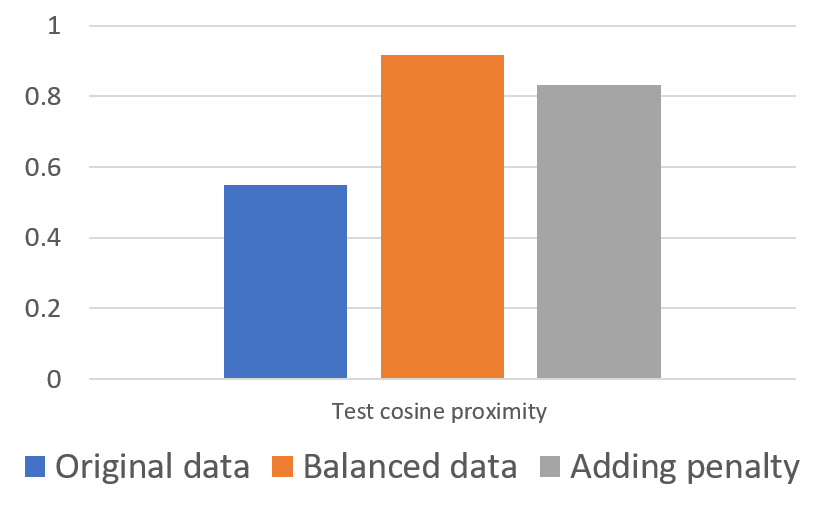
\includegraphics[width=0.9\linewidth]{figures/acc_f1_comp_ip_reg.png}
    \caption{Result on LSTM regression with different input.}
    \label{result_acc_f1_comp_ip_reg}
\end{figure}

$$\alpha = \frac{1}{10+{\rm Total~votes}}$$

Basically, the less votes, the lower score it will be. 

The results are shown in Fig. \ref{result_acc_f1_comp_ip_reg}. The training on the original dataset yields moderate correlation between the predicted scores and the true scores. However , when we remove the 0-vote reviews (balanced data case in the figure), the correlation coefficient boosts to 0.91, which indicates very strong statistical correlation and we can predict accurate helpfulness score without the noises in the dataset. However, we also observed that adding penalty will reduce the cosine proximity by 10\% from the previous case.  Overall, the LSTM model in predicting helpfulness score is promising.

\subsection{Convolutional Network Classification Results}

We implement a convolutional neural network model described in method following the structure talked in \cite{kim2014cnntext} and \cite{cnnimplement}.

\begin{figure}[tbp]
    \centering
    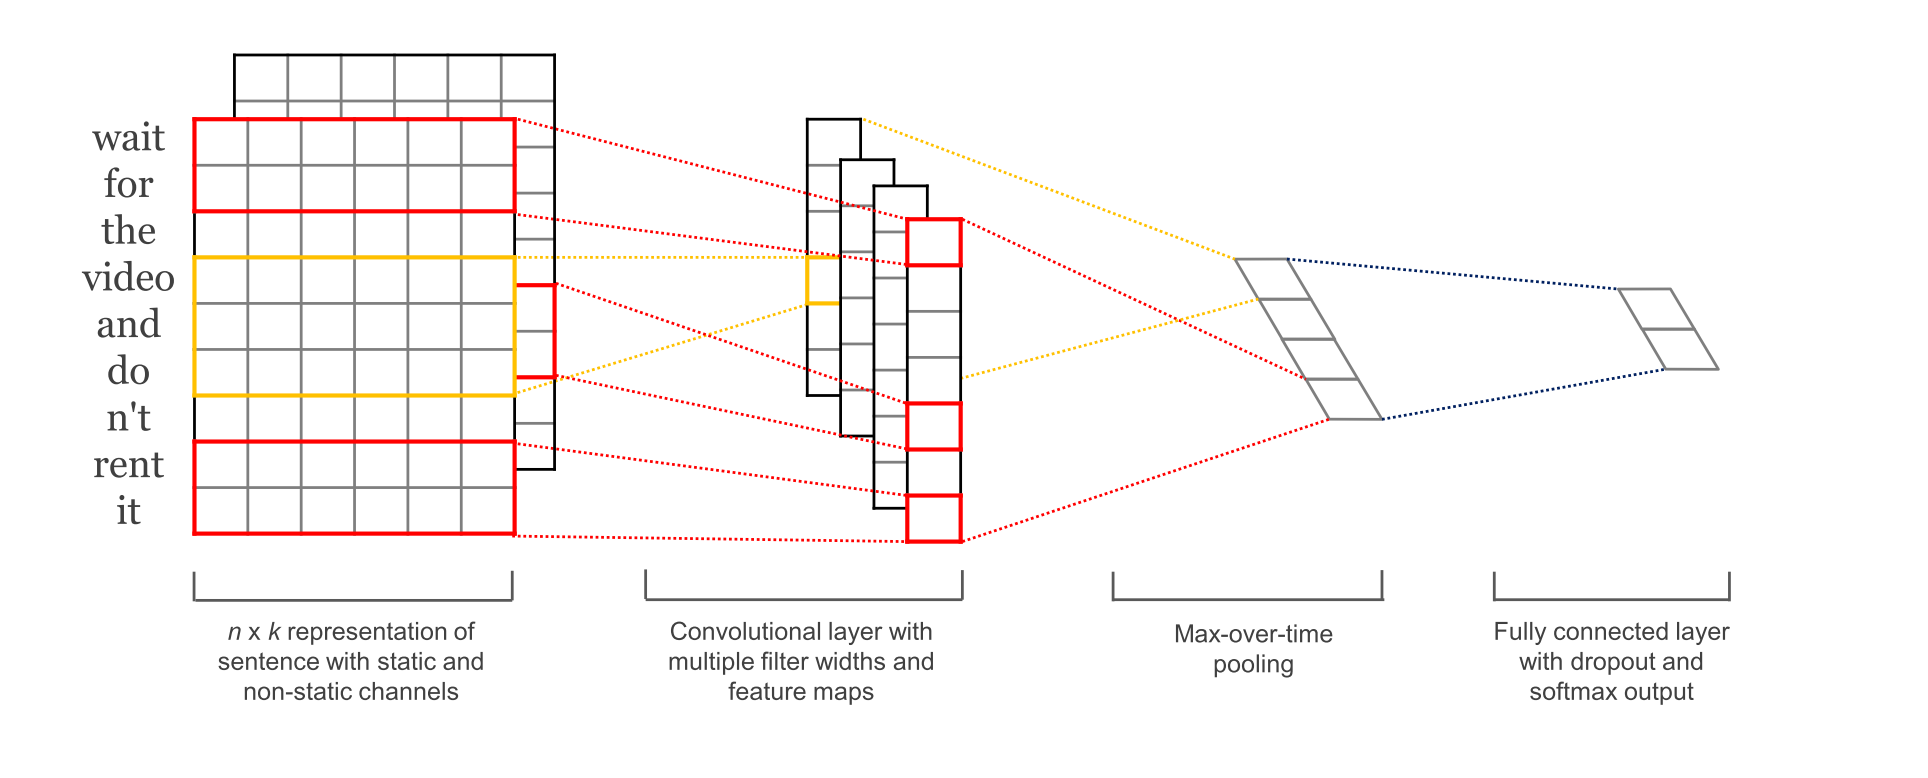
\includegraphics[width=0.9\linewidth]{CNN_structure.png}
    \caption{The structure of convolutional neural networks in our implementation.}
    \label{fig:cnn}
\end{figure}

Our convolutional neural network structure is displayed on Figure \ref{fig:cnn}. We first use embedding method to convert a sentence into a matrix (We also use simple vector without embedding as input). The convolutional filter applied on input matrix with different window size \(h\). In most of our experiment, we use 3, 4, and 5 as our window sizes. For each window size, we have 128 filters, so that it will generate 128 features for each window in our sequence. A max pooling layer will choose the max value of the feature in the sequence and output 128 value (feature). The features then are processed by a fully-connected layer to generate the prediction. The optimizer we used is Adam optimizer with initial learning rate \(1\times 10^{-4}\).

For the experiment, we test several different setups:

\textbf{Simple Model:} Our baseline model is using word token directly without embedding and without \(l_2\) norm regularization on the loss function.

\textbf{\(l_2\) regularized model:} We add \(l_2\) norm regularization on the loss function compared to the simple model.

\textbf{More filters model:} Instead using the windows size of 3, 4, and 5, we follow the setup of the discriminator in SeqGAN model \cite{yu2017seqgan}. So there are 10 different window size in this model.

\textbf{GloVe embedding model:} As described before, we use embedding model (GloVe pretrained model) to convert token into vector. And our input of CNN is a matrix for this case.

\textbf{3X data model:} Beside using GloVe embedding, we also use larger dataset for this model.

\begin{figure}[tbp]
    \centering
    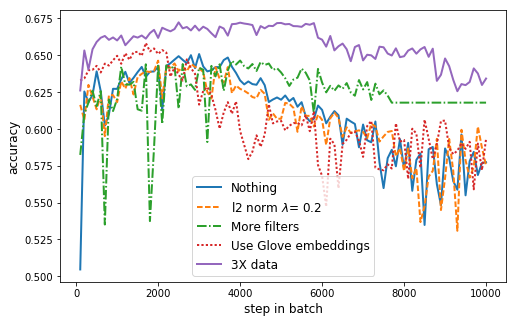
\includegraphics[width=0.9\linewidth]{CnnResultTrain.png}
    \caption{The test accuracy of different CNN model with different training steps.}
    \label{fig:cnn_result}
\end{figure}

The training performance of the CNN models is shown in Figure \ref{fig:cnn_result}. We can found that most of the models tend the to overfit very quickly. As after certain step, the test accuracy is decreasing although training accuracy still high (Not showing in the figure). Adding \(l_2\) norm regularization term not resolve the problem. The larger data size of input does improve the training as the test accuracy start to drop at the later stage.

\begin{figure}[tbp]
    \centering
    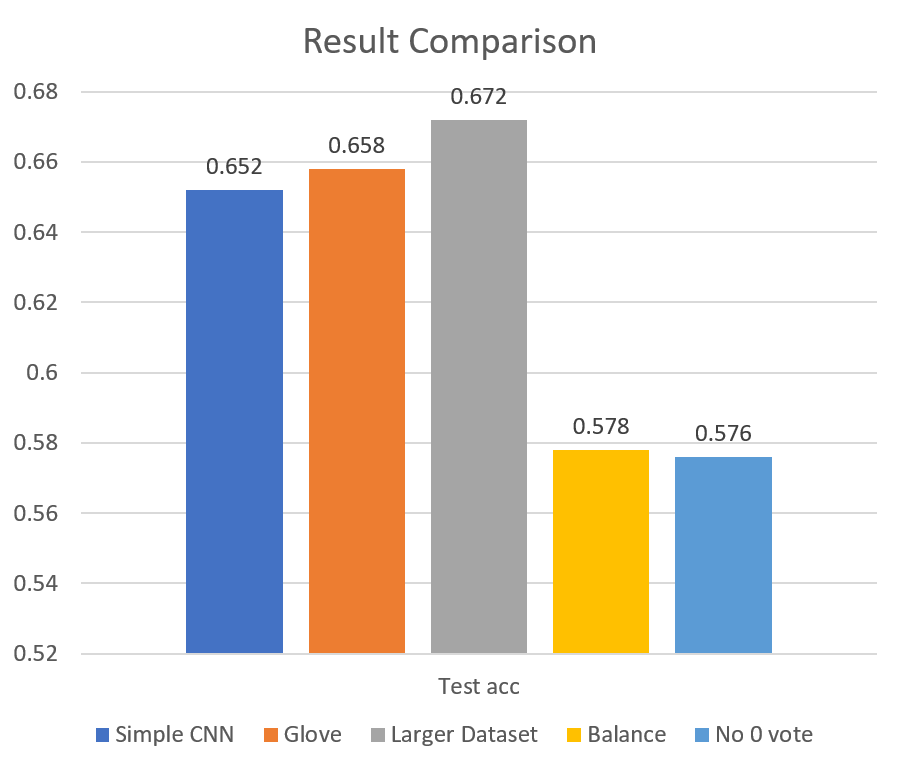
\includegraphics[width=0.9\linewidth]{CnnResult.png}
    \caption{The comparison of best test accuracy for different model and input dataset.}
    \label{fig:cnn_result_2}
\end{figure}

Comparing the best test accuracy achieved in our models in Figure \ref{fig:cnn_result_2}. For simple CNN model, the best accuracy is about 65\%. By using word embedding, the result got 1\% boost. The larger size of input dataset helps the model achieve another 1\% accuracy improvement. We also considered that the input data set is unbalanced, so we limit the size of input of each label to make it a balanced dataset. The test accuracy becomes around 58\%. We also consider the 0 vote reviews may also have features that belong to helpful or not helpful reviews. So we exclude 0 vote reviews in another test. However, the test accuracy not improved, suggesting 0 vote reviews may not cause any confusion for compare features.

\section{Discussion}

There are several issues we would like to address here.

First of all, one thing we would like to claim is that, the reason we use fixed 256 sequence length is that the average sequence length in our corpus is around 147. Only minority of the data has length longer than 256. However, this does not mean that we can not differentiate the length of each review. Because in vectorization process, those shorter sentence are padded to 256 by adding 0 vectors, which tells the model there is nothing in this slot, and they will not making contribution to the state transition within the recurrent layer.

Second, in our experiment, we only use text as our input to predict the helpfulness of reviews. In fact, other features of the review, like score, and whether the review has image, may also help to generate correct prediction. So maybe we can use neural networks to extract features from text, then combine other features as input for common classifier like Random Forest to further improve our predict accuracy.

Third, in the evaluation of LSTM model, we compare the performance of the model by using multiple cases. One significant observation is that, the 0-vote reviews plays an important role in the model performance. We consider it as noise because some truly helpful or unhelpful reviews are hidden because no customer give it a vote. Thus it fuzzifies our ground truth. Removal of such review boost the model performance significantly. 

Fourth, In our CNN experiment, we only use one convolutional layer. It is possible that a more complex network structures may also help the prediction, but may facing the challenge of overfitting. It is also possible that use CNN extract features the use LSTM to process the sequences of features to generate better prediction. However, the best performance of CNN model actually outperforms LSTM by 4\% in the original dataset, which makes it a good substitution in sequence processing with vectorization. Actually we can think of the convolutional filter can serve as a bigram, trigram or quadgram scanner, thus it has ability to extract the word dependency.

Finally, it is hard for us to understand what contributes to a helpful or unhelpful review because ``reverse engineering'' is almost impossible for sequential data processing by neural network. Because the outputs of the recurrent hidden layers are usually abstract number extracted from the embedded matrix. Meanwhile, although CNN is proven to be able to extract feature from images, the actually features extracted from sequence matrix are unreadable. In a word, we can not know what semantic feature a helpful or unhelpful review possess. To analyze this, we can use traditional bag-of-words method to count the TD-IDF and find out the high ranking terms in the review samples. We leave this to the future work. 

\section{Conclusion}

In this paper, we manage to employ the popular deep network such as LSTM and CNN as our model to predict the helpfulness of Amazon electronics product reviews. We first address the importance of helpfulness analysis, then we review some of the recent work that try to solve this problem. Later we propose our LSTM model and CNN model and their preprocessing techniques. Extensive experiments are conducted to explore the effectiveness of data size, preprocessing and input data quality. We find out that both larger data set and correct preprocessing help to improve the test accuracy. What's more the precision of the ground truth is essential in improving the performance. 

Different models are also evaluated, CNN actually outperforms LSTM-based RNN slightly, which indicates that CNN can be a substitution for RNN in some sequence processing applications. Our LSTM regression model has great performance in the balanced dataset. 

However, there are many interesting topics that we can explore, such as what contributes to a helpful or unhelpful reviews and whether stop word removal or word stemming would help to improve the test results. These question will be left for the future. 

\section{Acknowledgement}

Teamwork is appreciated along with the completion of the course project. Deliang will finish the data pre-processing part. Both of the two members will cooperate to build and test the deep network model. Deliang focuses on LSTM RNN part, Nan focuses on the CNN part. Both of the authors will work together on organizing the results for the presentation and the final report. 

The authors also want to thank Dr. Chai for valuable advice on improving this work.

\bibliographystyle{acl}
\bibliography{cse842final}

\end{document}